\section{Desenvolvimento do Memora}
\label{sec:desenvolvimento}

Esta seção apresenta os resultados das etapas que antecederam a implementação: a comparação dos simuladores e a escolha da base, o levantamento e a definição dos requisitos, a inspeção de usabilidade e o projeto do protótipo. A exposição relaciona o que foi observado às decisões adotadas para o Memora.

\subsection{Análise comparativa e escolha da ferramenta de base}

A análise considerou ferramentas relacionadas à memória cache que possuíam acesso gratuito ou acadêmico e documentação que permitisse caracterizar seus recursos. Foram incluídos simuladores visuais e ferramentas por linha de comando, para examinar diferentes formas de apresentar estados e resultados. A disponibilidade de código foi um critério para escolher a base a ser modificada, sem excluir da comparação ferramentas gratuitas cujo código público não foi identificado.



\label{sec:tabela-lacunas}

A Tabela~\ref{tab:comparacao-geral} sintetiza acesso, tecnologia e finalidade das ferramentas; a Tabela~\ref{tab:matriz-funcionalidades} compara seus recursos. Na matriz, \tem{} indica suporte identificado; \parcial{}, suporte parcial; e \nao{}, recurso não identificado.

\begin{table}[!htbp]
\centering
\caption{Características gerais das ferramentas selecionadas.}
\label{tab:comparacao-geral}
\footnotesize
\begin{tabular}{@{}P{2.3cm}P{4.2cm}P{7.6cm}@{}}
\toprule
\textbf{Ferramenta} & \textbf{Licença e acesso} & \textbf{Tecnologia e finalidade} \\
\midrule
Beto & Código aberto, MIT; web gratuito & HTML/CSS/JavaScript; visualização educacional em português. \\
ParaCache & Web gratuito; código público não identificado & Simulação educacional de cache e memória virtual. \\
Ripes & Código aberto, MIT & C++/Qt; arquitetura RISC-V, montagem e cache. \\
SMPCache & Gratuito/acadêmico; código público não identificado & Windows; cache em multiprocessadores. \\
Dinero IV & Fonte disponível; uso não comercial & C/linha de comando; análise por rastros e multinível. \\
Cache Simulator & Código aberto, MIT & Python/linha de comando; cache para MIPS. \\
QtMips & Código aberto, GPL-3.0 & C++/Qt; CPU MIPS, \textit{pipeline} e cache. \\
\bottomrule
\end{tabular}
\par\footnotesize Fonte: síntese da documentação das ferramentas apresentada na Seção~\ref{sec:relacionados}.
\par\bigskip


\centering
\caption{Funcionalidades identificadas na documentação das ferramentas.}
\label{tab:matriz-funcionalidades}
\footnotesize
\setlength{\tabcolsep}{4pt}
\begin{tabular}{@{}P{5.1cm}*{7}{c}@{}}
\toprule
\textbf{Recurso} & \textbf{Beto} & \textbf{ParaCache} & \textbf{Ripes} & \textbf{SMP} & \textbf{Dinero} & \textbf{Python} & \textbf{QtMips} \\
\midrule
Mapeamento direto & \tem & \tem & \tem & \tem & \tem & \tem & \parcial \\
Totalmente associativo & \tem & \tem & \tem & \tem & \tem & \tem & \parcial \\
Associativo por conjunto & \tem & \tem & \tem & \tem & \tem & \tem & \parcial \\
FIFO & \tem & \tem & \parcial & \tem & \tem & \nao & \parcial \\
LRU & \tem & \tem & \tem & \tem & \tem & \tem & \parcial \\
Aleatória & \tem & \tem & \parcial & \tem & \parcial & \nao & \nao \\
LFU/MRU ou política adicional & \nao & \nao & \parcial & \tem & \parcial & \tem & \nao \\
Operações \textit{load/store} & \nao & \tem & \tem & \tem & \tem & \parcial & \tem \\
Políticas de escrita & \nao & \tem & \tem & \tem & \tem & \nao & \parcial \\
Bit de validade & \parcial & \tem & \tem & \tem & \parcial & \parcial & \parcial \\
\textit{Dirty bit} & \nao & \tem & \tem & \tem & \parcial & \nao & \parcial \\
Estado LRU visível & \nao & \nao & \tem & \parcial & \nao & \nao & \nao \\
Decomposição do endereço & \parcial & \tem & \tem & \parcial & \parcial & \tem & \parcial \\
Histórico/rastro por acesso & \parcial & \tem & \tem & \tem & \tem & \tem & \parcial \\
Estatística/gráfico/exportação & \parcial & \tem & \tem & \tem & \tem & \parcial & \parcial \\
\bottomrule
\end{tabular}
\par\footnotesize SMP: SMPCache; Python: Cache Simulator. \tem{}: identificado; \parcial{}: parcial/a confirmar; \nao{}: não identificado. Fonte: síntese da documentação das ferramentas apresentada na Seção~\ref{sec:relacionados}.
\end{table}

O comparativo evidencia diferenças de finalidade. Dinero IV concentra-se na análise por rastros e não oferece interface gráfica; Ripes e QtMips articulam cache e execução de instruções. ParaCache reúne recursos de escrita em ambiente web, e SMPCache inclui coerência em multiprocessadores, mas não foi identificado código público dessas duas ferramentas. Ripes, por sua vez, combina recursos de análise com código aberto. Portanto, quantidade de funcionalidades e disponibilidade do código são dimensões distintas, que não permitem ordenar as ferramentas por uma única medida de qualidade.

O Beto reúne os três mapeamentos fundamentais e políticas clássicas em uma interface web em português. Em comparação com os recursos identificados nas demais ferramentas, sua apresentação pode tornar mais explícitos os estados de validade, a recência e a explicação de cada acesso. Escrita, modificação e simulação multinível representam ampliações do modelo funcional, distintas de ajustes de interface. 


O Beto foi selecionado por combinar acesso web gratuito, interface em português, licença MIT e código disponível. Além disso, já implementava os mapeamentos e as políticas necessários ao recorte de um nível de cache. Essas características permitiram preservar a base funcional e concentrar o desenvolvimento nas dificuldades de organização, ajuda e interpretação dos estados. As operações de escrita e a simulação de múltiplos níveis foram tratadas como ampliações do modelo, distintas dos ajustes de usabilidade priorizados.

\subsection{Levantamento e definição dos requisitos}
\label{sec:resultados-levantamento}

Com o intuito de definir quais melhorias seriam realizadas no Beto, foi elaborado um questionário com perguntas sobre o perfil dos estudantes, dificuldades de configuração e interpretação, problemas de usabilidade, melhorias desejadas e utilidade percebida. O instrumento está no Apêndice~\ref{ap:levantamento-beto}, com os enunciados, tipos de pergunta e alternativas de resposta. O formulário ficou disponível durante quatro semanas e recebeu 13 respostas de alunos de Engenharia de Computação que cursavam ou já haviam cursado as disciplinas relacionadas ao conteúdo. Todos concordaram com a participação voluntária e o uso anonimizado dos registros.

Os percentuais das perguntas de múltipla seleção foram calculados sobre as 13 pessoas que responderam. Por exemplo, cinco pessoas assinalaram dificuldade para compreender o significado dos campos, correspondendo a 38,5\%. Como cada pessoa podia escolher mais de uma alternativa na mesma pergunta, a soma dos percentuais dessas perguntas pode ultrapassar 100\%. Na análise, foram consideradas as seleções e as respostas abertas, sem tratar o número de marcações como uma ordenação das prioridades pelos participantes.

\paragraph*{Perfil dos respondentes.}
Os participantes possuem o seguinte perfil: sete declararam familiaridade avançada com memória cache, cinco intermediária e um básica. Nenhum indicou ausência de familiaridade. Quanto às disciplinas, seis cursavam AOC II e LAOC II, seis eram ex-alunos de uma ou de ambas e um cursava somente LAOC II. A Figura~\ref{fig:levantamento-perfil} apresenta essas distribuições.

\begin{figure}[!htbp]\centering
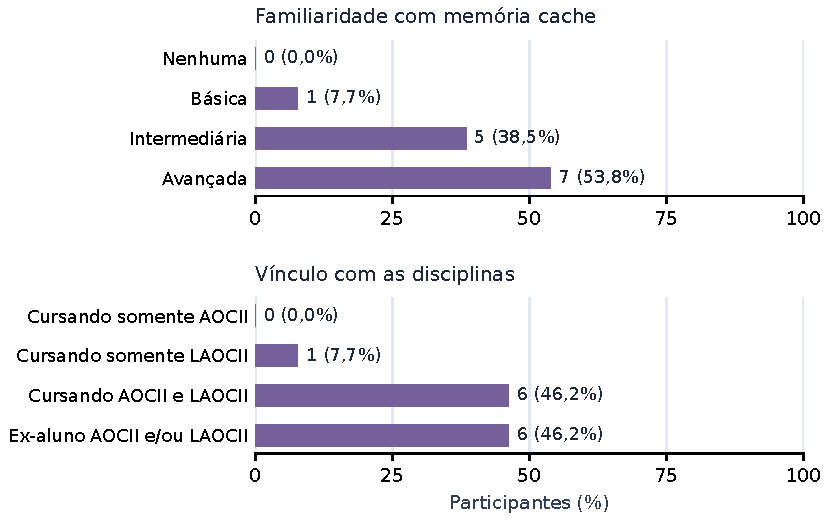
\includegraphics[width=\linewidth]{figuras/levantamento-perfil.pdf}
\caption{Perfil dos respondentes do levantamento de requisitos.}\label{fig:levantamento-perfil}
\par\footnotesize Fonte: elaboração própria a partir das 13 respostas.
\end{figure}

\paragraph*{Dificuldades na configuração.}
As dificuldades mais selecionadas foram compreender o significado dos campos e saber quais valores eram válidos, ambas assinaladas por cinco pessoas (38,5\%). Cinco também indicaram não ter encontrado dificuldades nessa etapa. As alternativas não são categorias exclusivas entre pessoas; representam o que cada respondente assinalou. A Figura~\ref{fig:levantamento-configuracao} apresenta todas as alternativas, incluindo o relato adicional de parâmetros incompatíveis e contagens fracionárias de bits.

\begin{figure}[!htbp]\centering
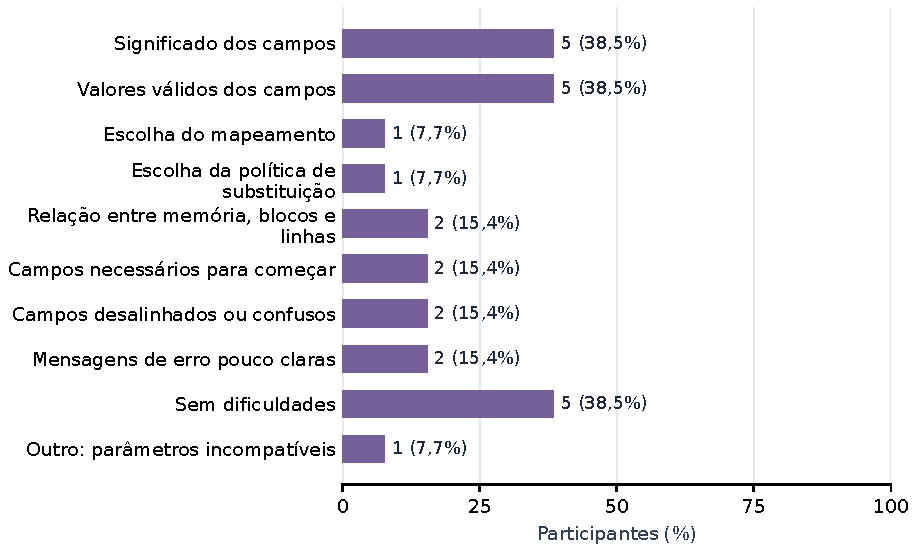
\includegraphics[width=\linewidth]{figuras/levantamento-configuracao.pdf}
\caption{Dificuldades encontradas durante a configuração do Beto.}\label{fig:levantamento-configuracao}
\par\footnotesize Fonte: elaboração própria; múltipla seleção, base de 13 respondentes.
\end{figure}

\paragraph*{Informações necessárias durante a simulação.}
A visualização da recência LRU por linha ou via foi a informação ausente mais selecionada: dez respostas (76,9\%). O bit de modificação foi assinalado por cinco pessoas (38,5\%) e o histórico passo a passo por três (23,1\%). A Figura~\ref{fig:levantamento-informacoes} reúne também os itens não selecionados, permitindo distinguir os recursos apontados pelos respondentes.

\begin{figure}[!htbp]\centering
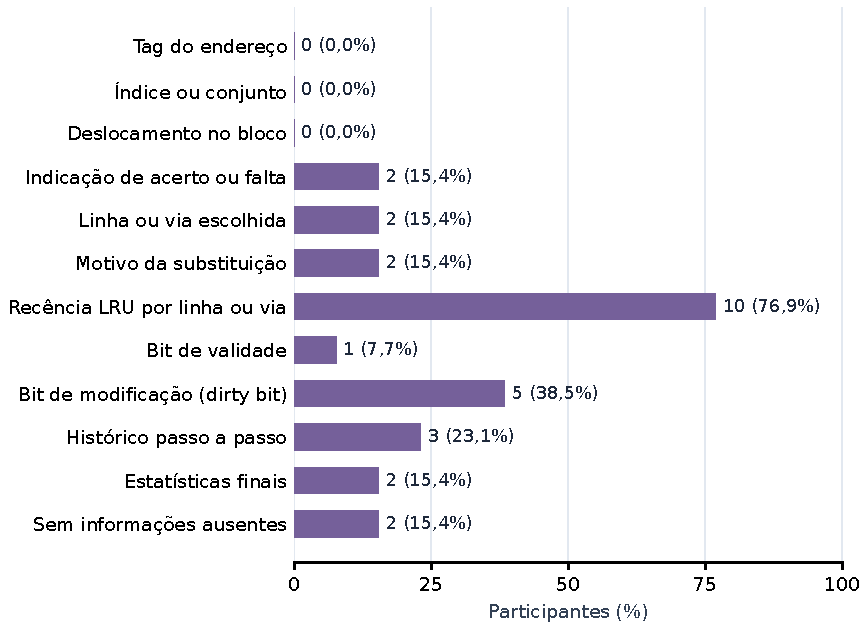
\includegraphics[width=\linewidth]{figuras/levantamento-informacoes.pdf}
\caption{Informações que os respondentes sentiram falta durante a simulação.}\label{fig:levantamento-informacoes}
\par\footnotesize Fonte: elaboração própria; múltipla seleção, base de 13 respondentes.
\end{figure}

\paragraph*{Problemas de usabilidade.}
O excesso de informação na tela foi indicado por oito pessoas (61,5\%). A ausência de ajuda, instruções ou documentação na interface recebeu cinco marcações (38,5\%). Falta de retorno após uma ação e mensagens pouco claras tiveram quatro marcações cada (30,8\%). Esses resultados, apresentados na Figura~\ref{fig:levantamento-usabilidade}, indicaram a necessidade de organizar a apresentação e aproximar explicações e mensagens dos elementos em uso.

\begin{figure}[!htbp]\centering
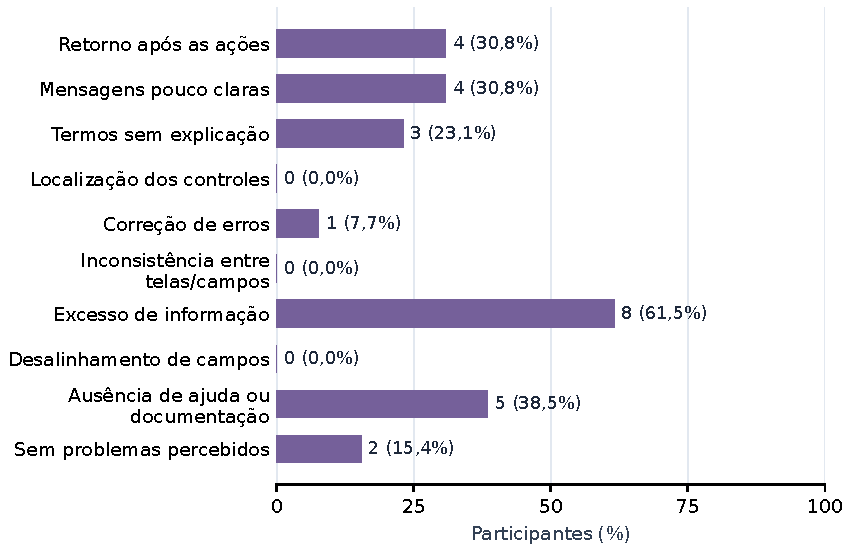
\includegraphics[width=\linewidth]{figuras/levantamento-usabilidade.pdf}
\caption{Problemas de usabilidade percebidos no Beto.}\label{fig:levantamento-usabilidade}
\par\footnotesize Fonte: elaboração própria; múltipla seleção, base de 13 respondentes.
\end{figure}

\paragraph*{Melhorias indicadas pelos usuários.}
As três alternativas mais selecionadas foram exibir a recência LRU, com dez respostas (76,9\%), melhorar a ajuda ou documentação, com nove (69,2\%), e incluir bit de modificação e políticas de escrita, com oito (61,5\%). Operações de leitura e escrita, explicação dos termos e mensagens de erro didáticas receberam sete marcações cada (53,8\%). A Figura~\ref{fig:prioridades-beto} apresenta as 15 alternativas. Essas frequências foram consideradas junto das dificuldades relatadas e dos objetivos do trabalho na definição do escopo.

\begin{figure}[!htbp]\centering
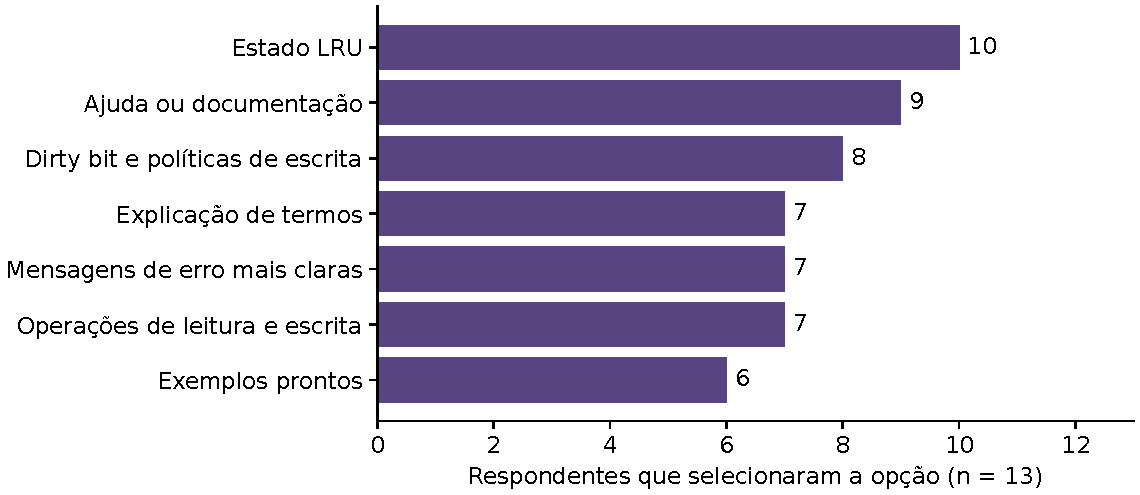
\includegraphics[width=\linewidth]{figuras/prioridades-beto.pdf}
\caption{Melhorias que os usuários indicaram como importantes para uma nova versão.}\label{fig:prioridades-beto}
\par\footnotesize Fonte: elaboração própria; múltipla seleção, base de 13 respondentes.
\end{figure}

\paragraph*{Respostas às questões abertas.}
Oito pessoas preencheram a pergunta aberta sobre melhorias adicionais. Os relatos abordaram o gerador de endereços aleatórios, a validação dos parâmetros, a leitura das informações e a indicação de término. O gerador permite criar a sequência de endereços que será acessada na simulação; foram relatados perda de funcionamento após editar essa sequência manualmente e travamento ao solicitar uma quantidade muito grande de endereços.

Também foram relatados travamento ao inserir zero na quantidade de palavras por bloco e dificuldade com combinações incompatíveis de parâmetros. Em particular, uma resposta descreveu valores fracionários na quantidade de bits exibida para \textit{tag} e conjunto na área de detalhamento. Trata-se da contagem de bits apresentada pela interface após a configuração, e não de um novo campo que deva receber valores fracionários. Esses relatos orientaram a validação antecipada e mensagens que explicam quais combinações são aceitas.

Outras sugestões incluíram manter os cabeçalhos do histórico visíveis durante a rolagem, explicar o cálculo dos campos de endereço, tornar mais clara a relação com a memória principal e comunicar o término e o reinício. Esses pontos foram considerados na organização da interface, na ajuda contextual e no controle de estados da nova versão.

\paragraph*{Utilidade percebida do Beto.}
A Figura~\ref{fig:levantamento-utilidade} mostra as respostas sobre a utilidade do Beto para apoiar o entendimento de memória cache, em uma escala de 1 a 4. Nove pessoas assinalaram 4 (69,2\%) e quatro assinalaram 3 (30,8\%); não houve marcações em 1 ou 2. A apreciação favorável foi considerada junto das dificuldades: os estudantes reconheciam a utilidade da ferramenta e indicavam aspectos de sua apresentação e operação que poderiam ser melhorados.

\begin{figure}[!htbp]\centering
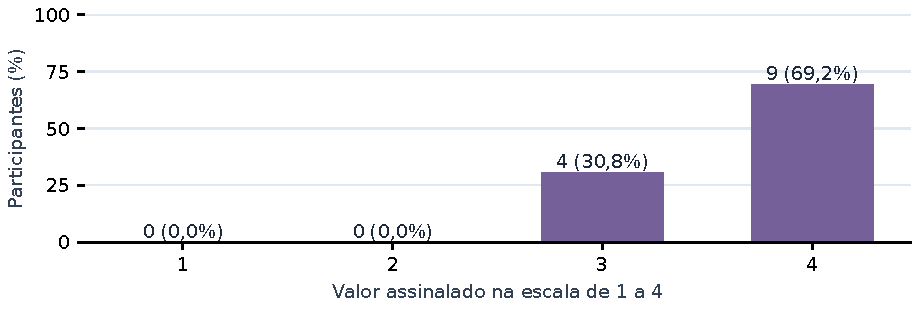
\includegraphics[width=.94\linewidth]{figuras/levantamento-utilidade.pdf}
\caption{Respostas sobre a utilidade do Beto para apoiar o entendimento de memória cache.}\label{fig:levantamento-utilidade}
\par\footnotesize Fonte: elaboração própria a partir das 13 respostas.
\end{figure}

\FloatBarrier
\paragraph*{Síntese e definição das prioridades.}
A análise mostrou demandas por novas operações e, simultaneamente, problemas de organização, explicação, validação e visibilidade do estado. A escolha das melhorias considerou a frequência das seleções, as dificuldades nas respostas abertas, a relação com o objetivo de usabilidade e o esforço de alteração do modelo de simulação.


Foram priorizadas a prevenção de configurações inválidas, a organização e a ajuda na interface, a visualização dos metadados e a revisão dos acessos. Essas melhorias atendem demandas frequentes e podem ser desenvolvidas preservando o modelo de um nível de cache. A tabela de prioridades foi organizada em quatro grupos de implementação (Tabela~\ref{tab:escopo-memora}); a numeração sistematiza a decisão do projeto e não representa uma classificação atribuída pelos respondentes.

A ordem de desenvolvimento partiu da configuração válida dos cenários, necessária para interpretar os resultados. Em seguida, foram organizados os campos e as explicações, que dão acesso às informações da simulação. A explicitação dos metadados e a revisão dos estados completaram esse fluxo. Assim, a ordem articula as necessidades relatadas às dependências entre as partes da ferramenta.

As operações de leitura e escrita foram indicadas por sete estudantes (53,8\%) e o bit de modificação e políticas de escrita por oito (61,5\%). Sua implementação exigiria ampliar o modelo de operações e a atualização da memória principal, além da interface. Considerando o prazo do TCC e o objetivo de melhorar a experiência de uso da base existente, essa ampliação foi reservada para trabalhos futuros. O levantamento, portanto, orientou tanto as melhorias escolhidas quanto a explicitação das demandas que ficaram fora desta entrega.

\begingroup\small
\begin{longtable}{@{}P{2.15cm}P{4.0cm}P{3.85cm}P{3.6cm}@{}}
\caption{Prioridades definidas para o desenvolvimento do Memora.}\label{tab:escopo-memora}\\
\toprule\textbf{Prioridade} & \textbf{Requisitos agrupados} & \textbf{Evidências do levantamento} & \textbf{Encaminhamento}\\\midrule\endfirsthead
\toprule\textbf{Prioridade} & \textbf{Requisitos agrupados} & \textbf{Evidências do levantamento} & \textbf{Encaminhamento}\\\midrule\endhead
1 & Validar entradas, explicar erros e limitar solicitações excessivas. & Mensagens didáticas: 7/13; validação: 4/13; relatos de travamento e parâmetros incompatíveis. & Implementar antes da execução e durante a edição.\\\midrule
2 & Reorganizar informações e oferecer ajuda, Glossário e explicação dos termos. & Ajuda: 9/13; termos: 7/13; excesso de informação: 8/13. & Implementar no fluxo de configuração e simulação.\\\midrule
3 & Explicitar decomposição, validade e recência LRU. & LRU: 10/13; decomposição: 2/13; validade: 2/13 nas melhorias. & Apresentar o estado utilizado pelo modelo existente.\\\midrule
4 & Oferecer histórico e comparação por acesso, controles claros e exemplos. & Exemplos: 6/13; histórico ausente: 3/13; relatos sobre término, reinício e explicações. & Implementar o acompanhamento e a revisão da simulação.\\
\bottomrule
\end{longtable}
\endgroup
\subsection{Inspeção de usabilidade}
\label{sec:inspecao-usabilidade}

A inspeção teve caráter qualitativo e utilizou as heurísticas de Nielsen como referência para examinar a interface, articulando o uso do Beto às dificuldades registradas no levantamento de requisitos. O exame percorreu a configuração dos parâmetros, a leitura da divisão do endereço, o acompanhamento da execução e a interpretação da memória cache. Em cada parte, foram considerados a informação necessária para a tarefa, a ação oferecida e o retorno comunicado ao usuário.

Entre os princípios examinados estão visibilidade do estado, correspondência entre os termos e os conceitos da disciplina, controle do usuário, consistência, prevenção de erros, reconhecimento, flexibilidade, concisão, recuperação de erros e ajuda \cite{nielsen1994heuristics}. Por exemplo, ao configurar uma memória, verificou-se se as restrições dos valores eram compreensíveis e se uma entrada incompatível recebia orientação; durante a execução, examinou-se como eram apresentados o acesso atual, o resultado e a escolha de uma linha ou via.

O diagnóstico foi consolidado nos aspectos apresentados na Tabela~\ref{tab:inspecao-usabilidade}. O levantamento com estudantes e a inspeção se complementaram: o primeiro registrou dificuldades relatadas, enquanto a inspeção relacionou essas dificuldades aos elementos da interface e às possibilidades de reformulação. O procedimento foi descritivo, sem atribuição de pontuações numéricas de severidade.

\begin{longtable}{@{}P{3.0cm}P{5.7cm}P{5.1cm}@{}}
\caption{Aspectos do diagnóstico de usabilidade e decisões para a nova interface.}\label{tab:inspecao-usabilidade}\\
\toprule\textbf{Aspecto examinado} & \textbf{Problema ou necessidade identificada} & \textbf{Decisão de projeto}\\\midrule\endfirsthead
\toprule\textbf{Aspecto examinado} & \textbf{Problema ou necessidade identificada} & \textbf{Decisão de projeto}\\\midrule\endhead
Organização das informações & A concentração de parâmetros, detalhamento e execução dificultava distinguir as atividades. Heurísticas: estética e concisão; reconhecimento. & Agrupar parâmetros e sequência; separar Configurar e Simular; apresentar explicações conforme o contexto.\\\midrule
Termos e ajuda & Dificuldades para compreender campos e resultados indicaram necessidade de apoio junto à informação. Heurísticas: correspondência com os conceitos; ajuda e documentação. & Ajuda contextual, Glossário e exemplos que relacionam parâmetros ao cenário simulado.\\\midrule
Validação e recuperação & Os relatos de entradas incompatíveis e contagens fracionárias de bits indicaram retorno insuficiente na configuração. Heurísticas: prevenção e recuperação de erros. & Validar durante o preenchimento e informar, próximo ao campo, o problema e a correção esperada.\\\midrule
Visibilidade dos estados & A interpretação das substituições exigia explicitar a recência LRU e a relação entre o endereço e a cache. Heurísticas: visibilidade; reconhecimento. & Mostrar decomposição, linha/conjunto, validade e recência quando aplicável; explicar cada acesso.\\\midrule
Controle da execução & Acompanhar os acessos requer distinguir preparação, reprodução, pausa, avanço e conclusão. Heurísticas: controle e liberdade; flexibilidade. & Controles de reprodução e avanço, velocidade ajustável e indicação explícita de término.\\\midrule
Histórico & Os relatos solicitaram explicações e acompanhamento de estados anteriores, além dos totais finais. Heurísticas: visibilidade; reconhecimento. & Histórico por acesso e comparação da cache antes e depois, sem repetir a execução.\\
\bottomrule
\end{longtable}

\subsection{Prototipação e revisão por docentes}
\label{sec:prototipacao}

O protótipo foi elaborado a partir dos requisitos priorizados e do diagnóstico de usabilidade. Utilizou-se o Figma, ferramenta de projeto de interfaces que permite organizar telas, componentes e estados visuais e compartilhar o trabalho para revisão \cite{figmaDesign2026}. Foram representados os campos de configuração, os três mapeamentos, os estados de erro, os controles da execução, a memória cache, o histórico e os painéis de ajuda. Essas representações permitiram discutir a apresentação antes de implementar todos os comportamentos.

Adotou-se como referência o \textit{Simple Design System} (SDS), um sistema de projeto disponibilizado pelo Figma que reúne padrões de componentes, estilos e variáveis visuais \cite{figmaSds2026}. No Memora, essa referência orientou a padronização de campos, botões, cartões, espaçamentos e tipografia. As cores associadas a endereço, resultado e estado da cache foram adaptadas aos conceitos apresentados pelo simulador.

O projeto passou por revisão com a orientação e a coorientação, envolvendo docentes de Arquitetura de Computadores e de IHC. Os registros dessa revisão apontaram ajustes na organização das telas e na identificação das ações. As abas passaram a ter aparência semelhante à de um navegador, com destaque para a etapa selecionada. Campos de entrada e botões receberam formas distintas e controles de mesma função passaram a compartilhar aparência e posição coerentes.

As ajudas também foram simplificadas. Foram retirados cabeçalhos e balões redundantes, as explicações passaram a usar linguagem dirigida ao estudante e os conteúdos foram organizados em descrição e exemplo didático. A redução de caixas repetidas e a padronização dos fundos procuraram facilitar a leitura sem eliminar regras e exemplos necessários à compreensão.

As representações de Configurar e Analisar estão no Apêndice~\ref{ap:capturas-complementares}, nas Figuras~\ref{fig:figma-configurar} e~\ref{fig:figma-analisar}. O protótipo previa três etapas: Configurar, Simular e Analisar. Durante a implementação, a comparação antes/depois passou a integrar a etapa Simular, como ação do histórico. Essa alteração preservou a análise do acesso e reduziu a repetição de informações entre telas.

